% !TeX root = ../main.tex

\section{Background}

Hidden Markov models are useful when inferring a single unobserved process, but biological processes often involve multiple simultaneous hidden processes which can occur and at different time scales. For example, a preliminary observation of the killer whale dive data shown in figure (\ref{fig:data}) shows that the behavior of this killer whale changes between approximately hour-long periods of predominately short, shallow dives and long, deep dives. Leos-Barajas et al. encounter a similar issue when modeling the movement of a harbor porpoise in the North Sea, and use it as a motivating example when they introduce hierarchical hidden Markov models.

\begin{figure}[h!]
	\centering
	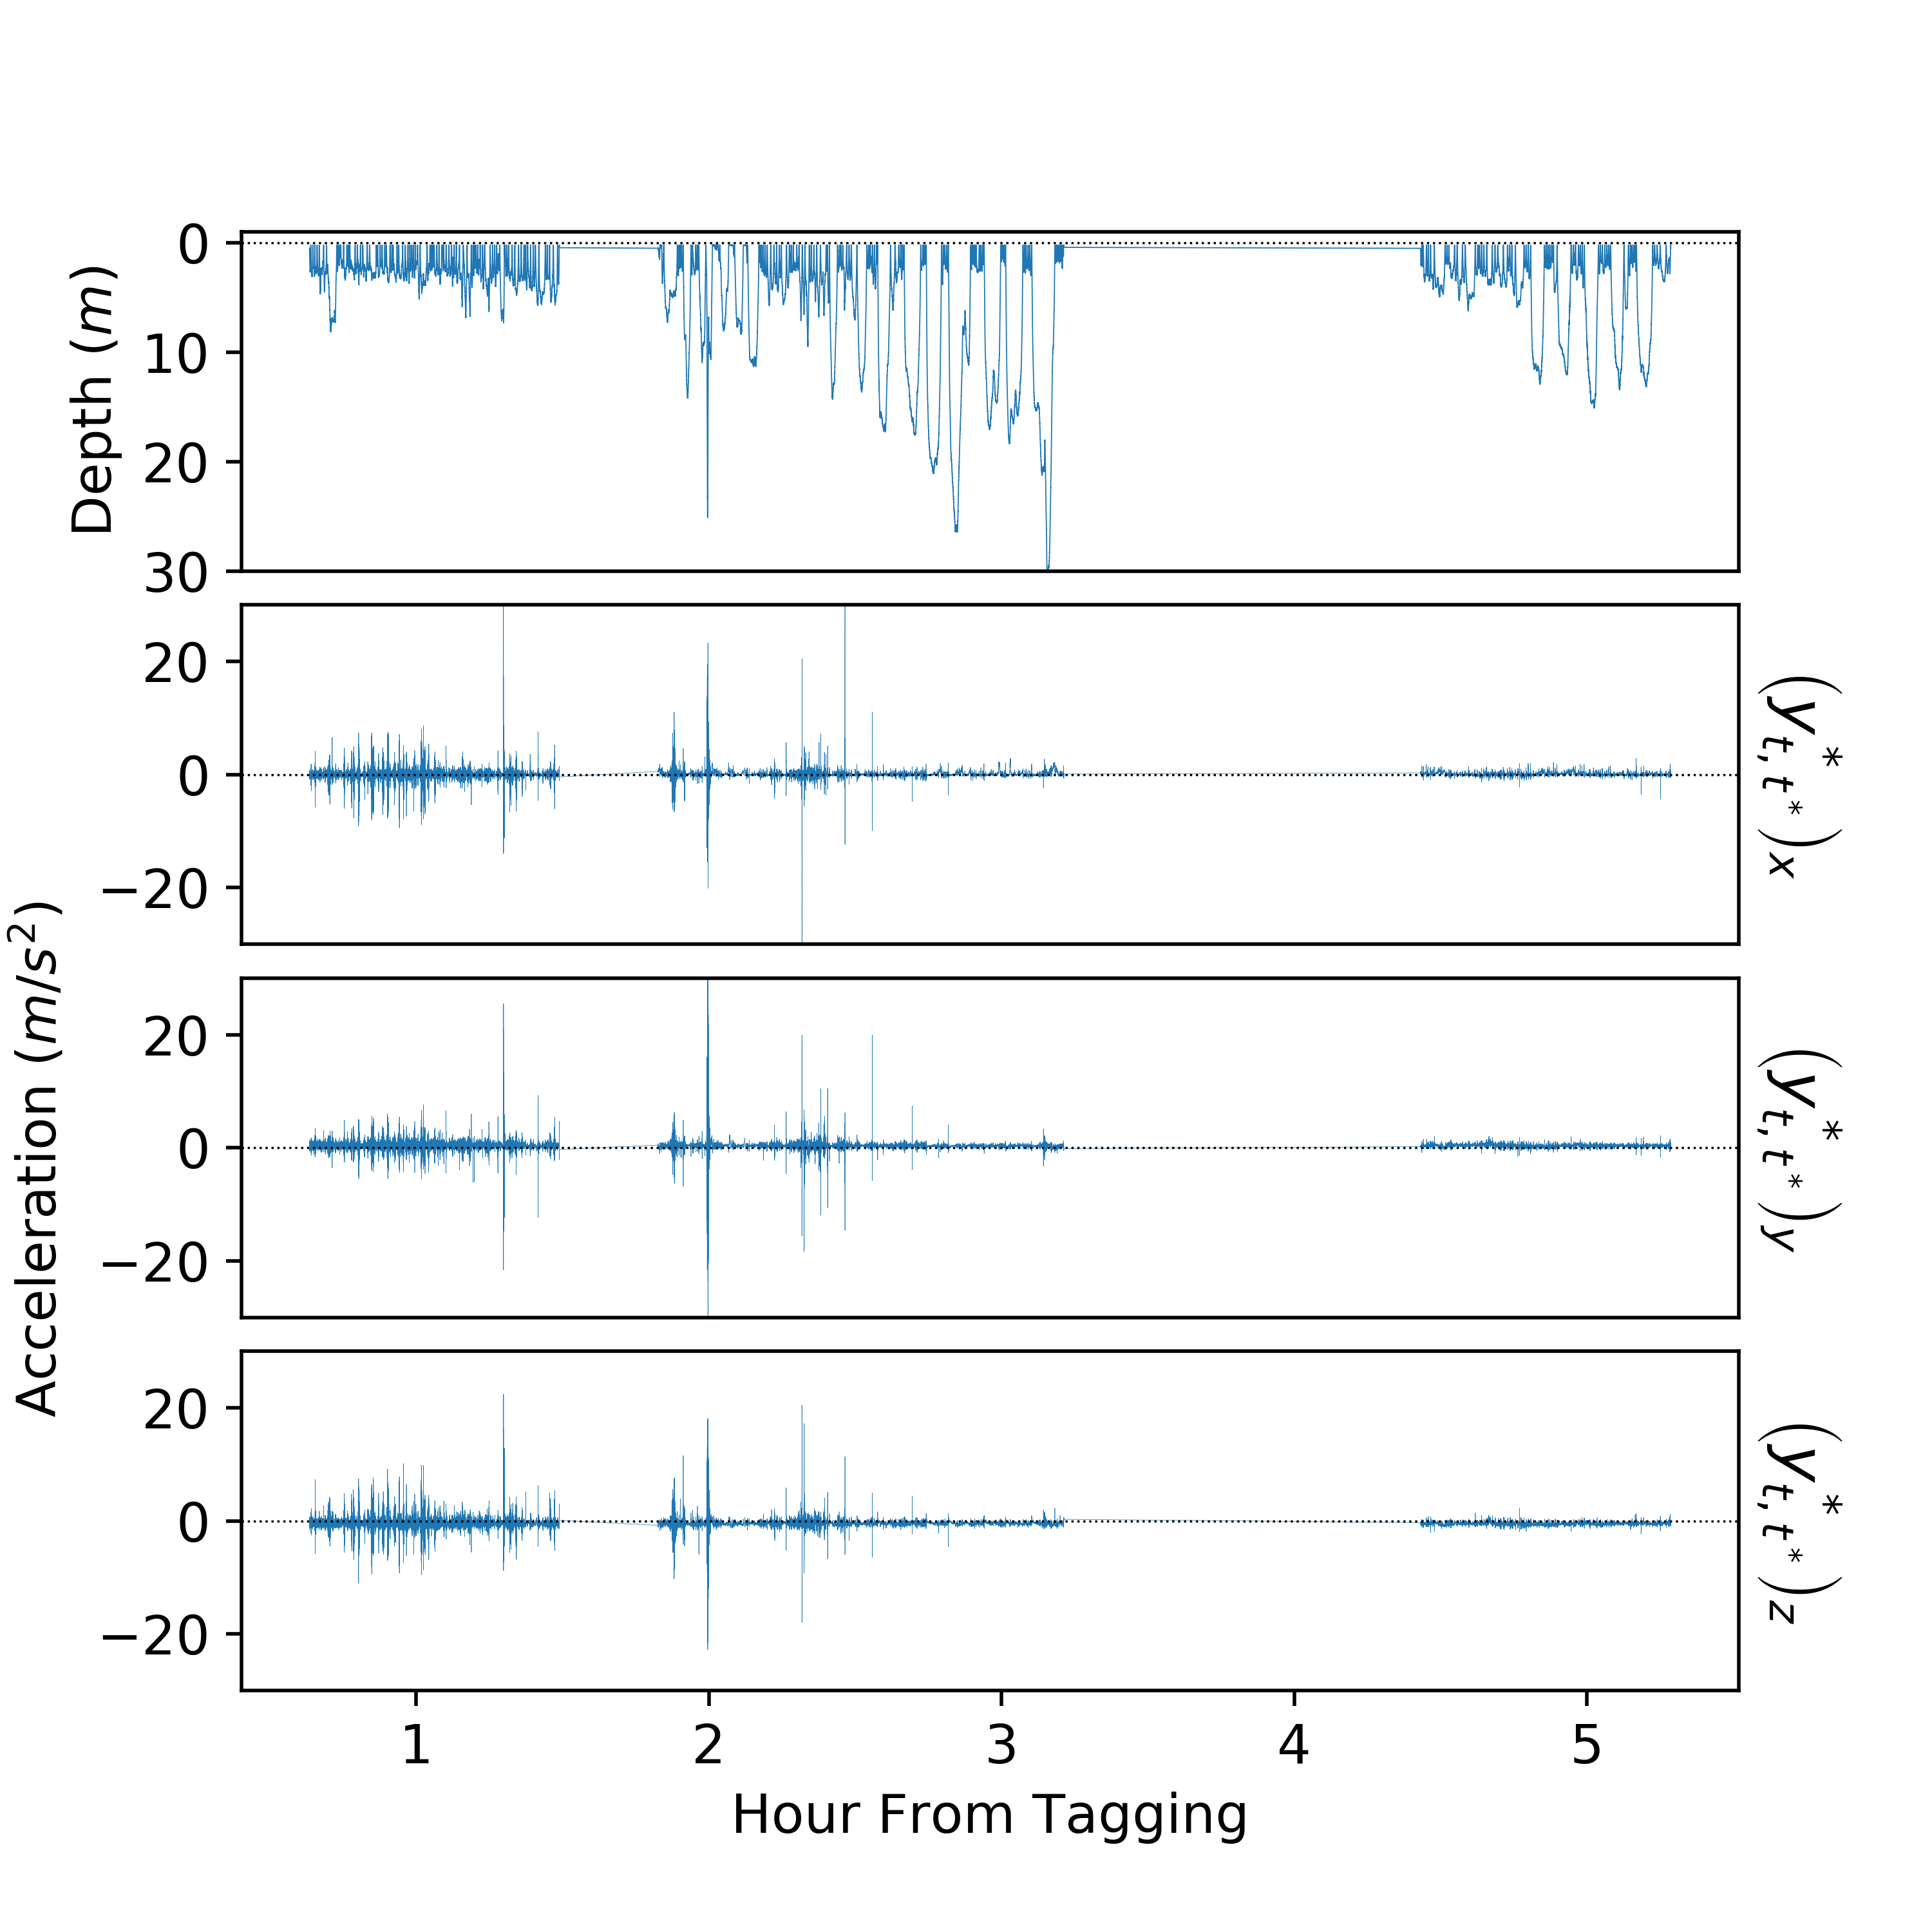
\includegraphics[width=6.5in]{../Plots/raw_data.png}
	\caption{Raw depth data of a Killer Whale off the coast of British Columbia, Canada.}
	\label{fig:data}
\end{figure}

\subsection{Hidden Markov models}

\textit{Hidden Markov models} (or HMMs) are comprised of an unobserved Markov chain $X = (X_1, \ldots, X_T)$ and a sequence of (possibly high-dimensional) observations $Y = (Y_1, \ldots, Y_T)$, each of length $T$. Each random variable in the unobserved chain $X_t$ can take one of $N$ possible values, and $X$ has corresponeding probability transition matrix $\Gamma \in \bbR^{N \times N}$ and initial distribution $\delta \in \bbR^N$:

$$\delta_i = Pr(X_1 = i)$$

$$ \Gamma_{ij} = Pr(X_{t+1} = j | X_t = i) \qquad \forall t \in \{ 1, \ldots, T-1\} $$

Further, each random varaible $X_t$ emits an observation $Y_t$ whose distribution depends only on the value of $X_t$ and none of the preceding observations or behavioral states: $p_{\theta}(y_t|x_t, x_{t-1}, \ldots , x_1, y_{t-1}, \ldots , y_1) = p_{\theta}(y_t|x_t)$. Note that the emission distribution depends upon parameters $\theta$. A visualization of this dependence structure can be seen in figure (\ref{fig:HMM}). In the field of animal movement, the unobserved chain $X$ usually represents the latent behaviour of an animal (e.g. foraging, resting, migrating, etc.), while the observations $Y$ are often a series of step lengths and turning angles for land animals and either depth or accelerometer data (or both) for marine animals.

The probability transition matrix $\Gamma$ and the parameters of the emission distributions, $\theta$, can be estimated by maximizing the likelihood of the observed data $y$, $\calL_{\text{HMM}}(y)$, with respect to the $\Gamma$ and $\theta$. In addition, $\calL_{\text{HMM}}(y)$ can be calculated using the \textit{forward algorithm}:
%
$$\calL_{\text{HMM}}(y;\theta,\Gamma,\delta) = \delta P(y_1;\theta) \prod_{t=2}^T \Gamma P(y_t;\theta) \mathbf{1}$$
%
where:
%
$$P(y_t;\theta) = \text{diag}(p_{\theta}(y_t|X_t = x_1), . . . , p_{\theta}(y_t|X_t = x_N ))$$
%
and $\mathbf{1}$ is an $N$-dimensional column vector of ones.

In order to enusre identifiability and right-stochasticity after optimizing $\calL_{\text{HMM}}(y)$, $\Gamma$ is parameterized using $\eta \in \bbR^{N \times N}$ and the following link function:

$$\Gamma_{ij} = \frac{\exp(\eta_{ij})}{\sum_{k=1}^N \exp(\eta_{ik})}, \qquad \eta_{ii} = 0 \quad \forall i \in \{1, \ldots, N\}$$

This allows for unconstrained optimization over $\eta$ and removes the constraint that $\Gamma$ be right-stochastic. $\calL_{\text{HMM}}(y;\theta,\Gamma,\delta)$ can be maximized using any numerical optimizer.

\begin{figure}[h!]
	\centering
	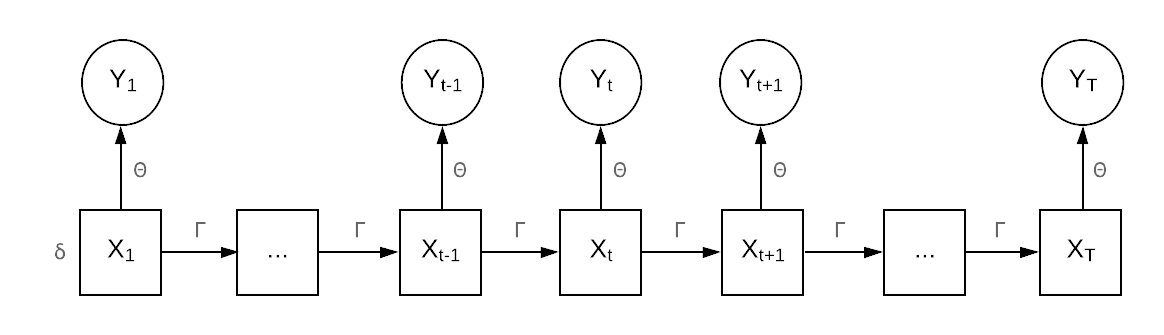
\includegraphics[width=3in]{../Plots/HMM.png}
	\caption{Graphical representation of a traditional HMM.}
	\label{fig:HMM}
\end{figure}


\subsection{Hierarchical HMMs}

A hierarchical hidden Markov model (or HHMM) is a variation of a hidden Markov model in which each hidden state of the original HMM $X_t$ emits both an observation $Y_t$ as well as another fine-scale hidden markov model of length $T^*_t$. This fine-scale HMM is comprised of a Markov chain $X^*_t = (X^*_{t,1}, \ldots, X^*_{t,T^*_t})$ and observations $Y^*_t = (Y^*_{t,1}, \ldots, Y^*_{t,T^*_t})$. As before, each fine-scale observation $Y^*_{t,t^*}$ depends only on the value of its corresponding hidden state, $X^*_{t,t^*}$. $X^*_{t,t^*}$ can take one of $N^*$ values and is characterized by an initial distribtuion $\delta^{*(X_t)} \in \bbR^{N^*}$ and probability transition matrix $\Gamma^{*(X_t)} \in \bbR^{N^* \times N^*}$:

$$\delta^{*(x_t)}_i = Pr(X^*_{t,1} = i | X_t = x_t)$$

$$\Gamma^{*(x_t)}_{ij} = Pr(X^*_{t,t^*+1} = j | X^*_{t,t^*} = i, X_t = x_t) \qquad \forall t^* \in \{ 1, \ldots, T^*_t-1\}$$

Finally, the fine-scale emission probabilities $p_{\theta^{*(X_t)}}(y^*_{s,t} | x^*_{s,t})$ are parameterized by $\theta^{*(X_t)}$. Note the parameters of the fine-scale hidden Markov model, $\Gamma^{*(X_t)}$, $\delta^{*(X_t)}$, and $\theta^{*(X_t)}$ all depend upon the hidden state of the \textit{crude-scale} hidden markov model. However, depending upon the discretion of the researcher, it is possible to force any of these parameters to be independent of the crude-scale hidden state $X_t$. A visualization of the full structure of the HHMM can be seen in figure (\ref{fig:HHMM}).

Due to the nested structure of a hierarchical hidden Markov model, the likelihood of an HHMM is still easy to calculate using the forward algorithm:
%
$$\calL_{\text{HHMM}}(y,y^*;\theta,\theta^*,\Gamma,\Gamma^*,\delta,\delta^*) = \delta P(y_1,y_1^*;\theta,\theta^*,\Gamma^*,\delta^*) \prod_{t=2}^T \Gamma P(y_t,y_t^*;\theta,\theta^*,\Gamma^*,\delta^*) \mathbf{1}$$
%
where:
%
\begin{align*}
	P(y_t,y_t^*;\theta,\theta^*,\Gamma^*,\delta^*)  = \text{diag}\left[p_{\theta}(y_t|x_t = x_1)\calL_{\text{HMM}}\left(y_t^*;\theta^{*(x_1)},\Gamma^{*(x_1)},\delta^{*(x_1)}\right), . . . , \right.\\
	\left. p_{\theta}(y_t|x_t = x_N )\calL_{\text{HMM}}\left(y_t^*;\theta^{*(x_N)},\Gamma^{*(x_N)},\delta^{*(x_N)}\right) \right]
\end{align*}
%
Note that this formualtion assumes that the crude-scale observations at a given time $Y_t$ and the fine-scale observation time series $Y_t^*$ are independent of one another when conditioned on $X_t$.

For more information on specific considerations for HHMMs such as incorporating covariates into the probability transition matrix, model selection and model checking, see Adam et al \cite{Adam:2019}.

\begin{figure}[h!]
	\centering
	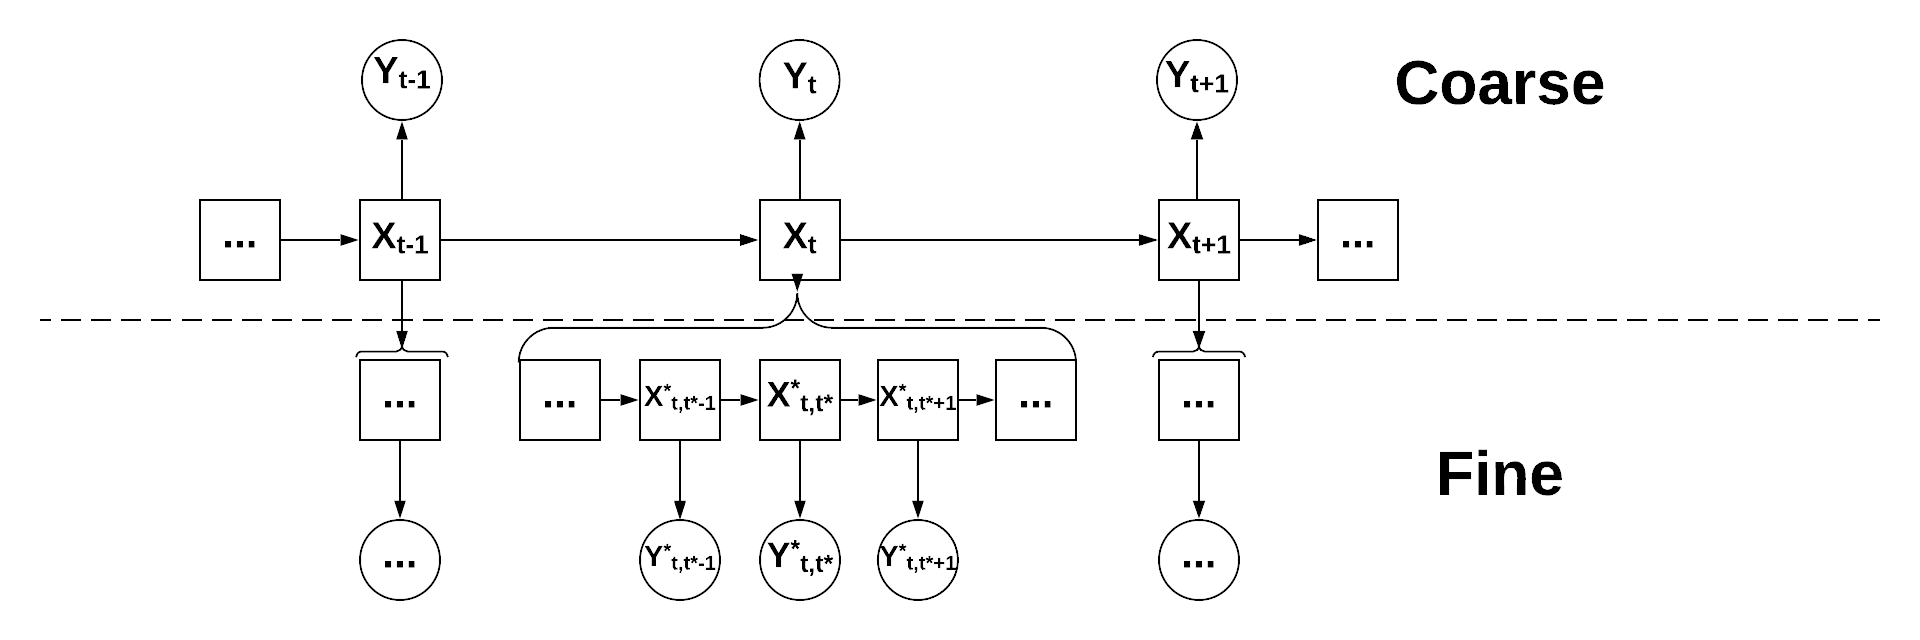
\includegraphics[width=6.5in]{../Plots/HHMM.png}
	\caption{Graphical representation of a traditional HHMM.}
	\label{fig:HHMM}
\end{figure}

\subsection{Conditionally autoregressive HMMs}

One of the key assumptions of both HMMs and HHMMs is \textit{conditional indpendence} between observations at both the crude and fine scale. Namely, given the state $X_t$ or $X^*_{t,t^*}$, $Y_t$ or $Y^*_{t,t^*}$ (respectively) is assumed to be independent from all other observations. Therefore, traditional HMMs and HHMMs can fail when the observation sequence $Y$ exhibits significant auto-correlation in time. Examples include fluking in marine mammals in Vancouver, BC (see the results section) and the swiming behavior of horn sharks off the coast of Southern California \cite{Adam:2019}.

One way to deal with autocorrelation in fine-scale behavioral processes is to use a state-switching continuous model such as the one introduced by Michelot et al \cite{Michelot:2019}, which models the movement of an animal as an Ornstein-Uhlenbeck process with parameters that depend upon the underlying behaviour state of the animal. Continuous time models are advantagous because of their flexibiliy: they can be built up from aribitrarily complex stochastic differential equations and they allow for uneven step lengths in the observations sequence $Y$. However, most continuous time models require MCMC algorithms to perform inference and as a result are not easily incorporated into the HHMM structure.

Another option is to use the CarHMM, or \textit{conditionally auto-regressive hidden Markov model}, introduced by Lawler et al \cite{Lawler:2019}, in which autocorrelation is explicity modeled into the emission distributions of the HMM while maintaining the strucutre needed to run the forward algorithm for fast direct likelihood maximization. In particular, if the emission distribution of observation $Y_t$ is parameterized by its mean and variance, i.e. $\theta_{x_t} = \{\mu_{x_t},\sigma^2_{x_t}\}$, the CarHMM introduces autocorrleation into the HMM by assuming that an observation $Y_t$ has mean $(1-\phi_{x_t}) \cdot \mu_{x_t} + \phi_{x_t} \cdot y_{t-1}$ rather than $\mu_{x_t}$. Note that the autocorrelation term $\phi_{x_t}$ depends upon the behavioral state of the animal. This model easily fits into the HHMM structure, but seems to lack the flexibility and natural interpretation of continuous-time models. However, we prove in the following section that under certain conditions these two models are in fact equivalent.

The likelihood of CarHMM is still compatible with the forward algorithm:
\begin{equation}
\calL_{\text{CarHMM}}(y) = \delta \prod_{t=2}^T \Gamma P(y_t;\theta) \mathbf{1}
\label{CarHMM_likelihood}
\end{equation}
where:
%
$$P(y_t;\theta) = \text{diag}(p_\theta(y_t|y_{t-1},X_t = x_1), . . . , p_\theta(y_t|y_{t-1},X_t = x_N )), \qquad t > 1$$
%
and the graphical model associated with the strcture of a CarHMM is shown in figure (\ref{fig:CarHMM}). Note that the first observation $y_1$ is assumed to be fixed as an initial value.

\begin{figure}[h!]
	\centering
	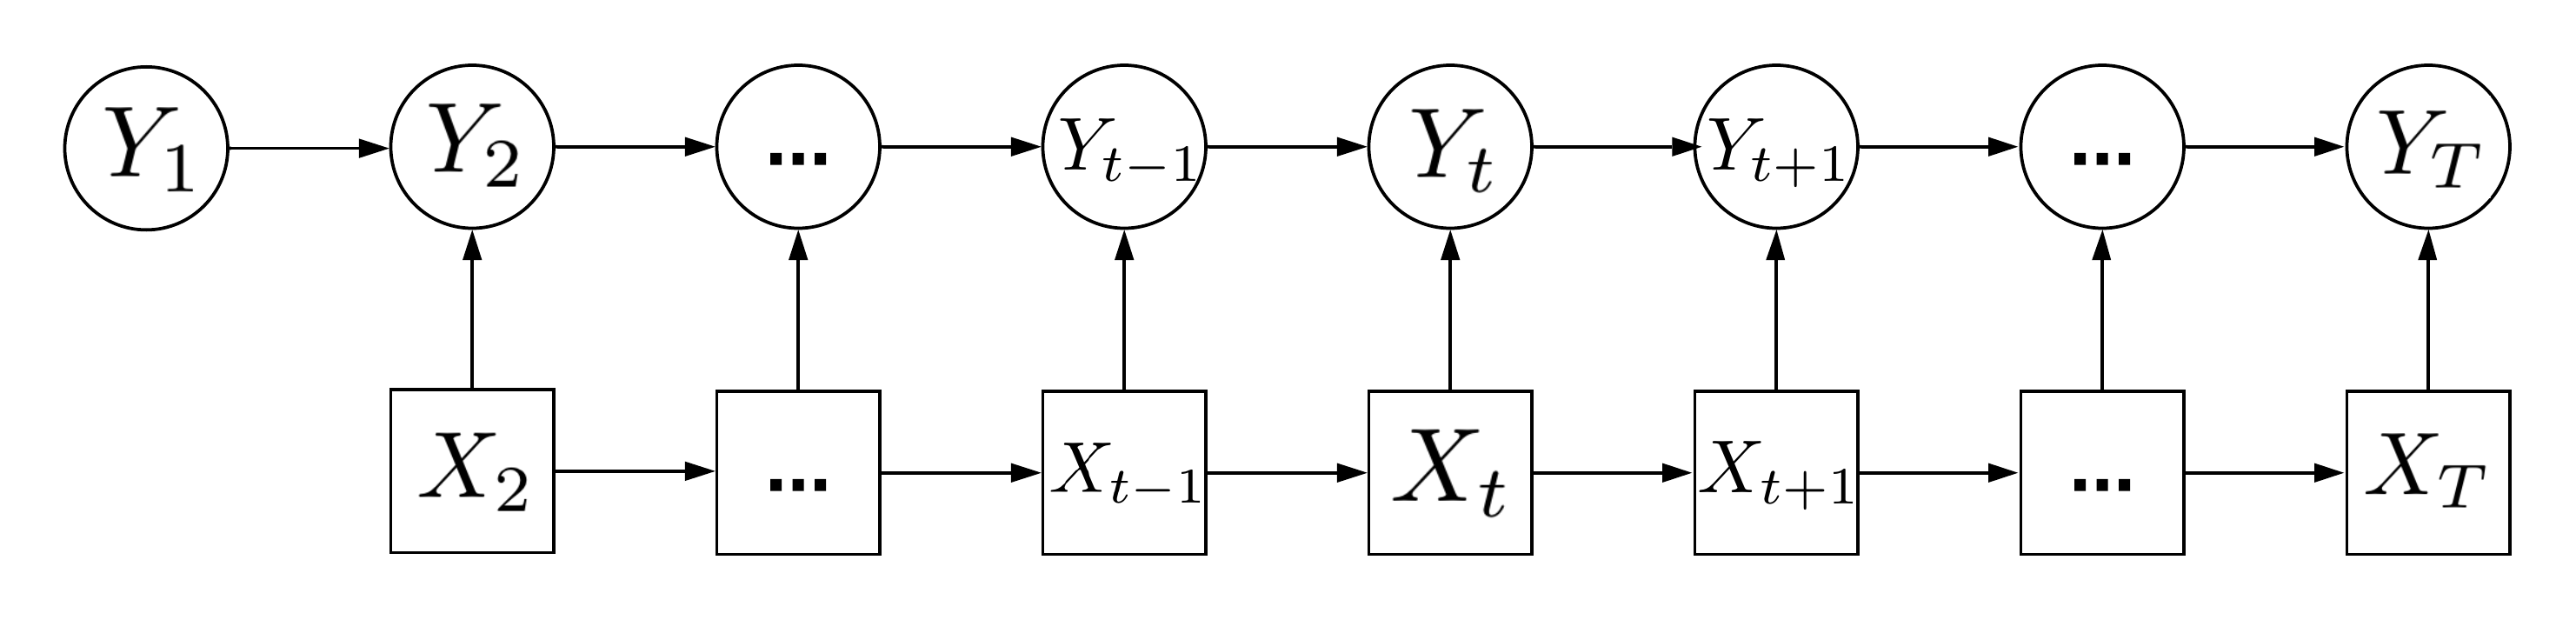
\includegraphics[width=3in]{../Plots/CarHMM.png}
	\caption{Graphical representation of a traditional CarHMM. The additional arrows representing autocorrelation between observations are shown in red for emphasis.}
	\label{fig:CarHMM}
\end{figure}



\subsection{State decoding}

Once an HMM, HHMM, or CarHMM model is fit using the process described above, it is common to find the most likely sequence of hidden states $\hat X$ conditioned on the learned parameters by using a dynamic programing algorithm called the Viterbi algorithm \cite{Viterbi:1967}. In the case of HHMMs, this can be followed by running the Viterbi algorithm again on each sub-dive state to find the mostly likely sequence of fine-scale hidden states $\hat X_t^*$ conditioned on the learned parameters and the estimated crude-state value $\hat X_t$. Note that while $\hat X$ is a maximum likelihood estimate of $X$, $\hat X^*_t$ is \textit{not} necessarily a maximum likelihood estimate of $\hat X^*_t$ because it is conditioned on the value of $\hat X_t$.

While the Viterbi algorithm is the de-facto standard in the current ecology literature, we suggest to instead find the \textit{probability} of each crude-level state (conditioned on the learned parameters) using the \textit{forward-backward algorithm}. The forward-backward algorithm has the same time complexity as the forward algorithm and is also used to find the \textit{psuedoresiduals} of a given model, which is an important tool for model validation. In addition, For HHMMs in particular, the forward-backward algorithm can be used recursively to find the probability of the fine-level states $X^*_{s,t}$ exactly by marginalizing out $X_t$:

$$P(X^*_{s,t} = x^*_{s,t}) = \sum_{n=1}^N P(X_t = x_n)P(X^*_{s,t} = x^*_{s,t} | X_t = x_n)$$

Where $P(X_t = x_n)$ can be found using the forward-backward algorithm on the crude-level markov chain and $P(X^*_{s,t} = x^*_{s,t} | X_t = x_n)$ can be found by running the forward-backward algorithm on the fine-level HMM for every possible value of $X_t$.

%\vspace{1cm}

%Model selection commonly involves the use of an information criterion such as the Akaike information criterion (AIC) or Bayesian information criterion (BIC). However, these metrics tend to favor complex models with more hidden states than can reasonably be interpreted in a biological setting [11]. While future studies may use non-parametric clustering techniques to find the number of crude-level and dive-level hidden states, Leos-Barajas et al. use exploratory analysis to determine their parameterization, and this work does the same.
%The timescale of the crude-scale Markov chain ideally should be short enough to ensure adequate resolution in the crude scale, but long enough so that the fine-scale Markov chains emitted by the crude-scale hidden Markov model are long enough to be informative. Because crude-scale behavioral changes occur on the time scale of approximately ten minutes, and there are a approximately thirteen dives per ten minutes of observation, this study uses a crude time scale of ten minutes. This differs from Leos-Barajas et al., who set the crude time scale to one hour.
%The killer whale in this study appears to be alternating between periods of mostly pre- dominately short, shallow, smooth dives and periods interspersed with long, deep dives. As a result, we set the number of crude states as K = 2. The number of possible dive types was set as N = 3 to allow for additional flexibility beyond long, deep dives and short, shallow dives. Gamma distributions were used for the emission probability density function because of their flexibility and that the observations are all non-negative. All of these decision follow the lead of Leos-Barajas et al.
%One additional assumption made both here and in the Barajas et al. paper is that
%the distribution of observations given a dive type is constant across all K crude-scale dive-
%level Markov chains. Mathematically this means that α(1) = ... = α(K) and β(1) = ... =
%3.3 Parameter Estimation and Likelihood Maximization
%Like the classical hidden Markov model, it is possible to use the forward algorithm to find the likelihood of an observed sequence of dives, Lw(y). The likelihood of the hierarchical model differs from the traditional HMM only in that the emission probability, p(y(t)|x(t)), is replaced by the likelihood of the fine-scale Markov chain at step m, Lx(y(m)|w(m)). Note that
%9
%(K)
%maximization algorithm.
%β
%. This assumption simplifies the model and facilitates convergence in the likelihood

%this likelihood depends upon the state of the crude-scale Markov chain, since the parameters
%dictating the dynamics of X
%K
%(m)
%(m)
%depend upon the value of W Lw(y) = 􏰚p(y(1:M),W(M) = wi)
%i=1 K
%. Formally:
%= 􏰚Lx(y(M)|W(M) = wi)p(y(1:M−1),W(M) = wi) i=1
%KK
%= 􏰚Lx(y(M)|W(M) = wi)􏰚P(wj → wi)p(y(1:M−1),w(M−1) = wj)
%i=1 j=1
%y(m) is a T(m)-by-R matrix of observations, Lx(y(m)|W(m) = wi) is the likelihood of one dive- level Markov chain given the crude behavioral state wi, and Lw(y) is the likelihood of the entire hierarchical model. Like in the traditional HMM model, this leads to the following recurrence relation:
%K
%p(y(1:m),W(m) =wi)=Lx(y(m)|W(m) =wi)􏰚P(wj →wi)p(y(1:m−1),W(m−1) =wj)
%j=1
%p(y(1), W (1) = wi) = δWwi ∗ Lx(y(1)|W (1) = wi)
%where δW is the initial distribution of crude-scale behavioral states. Again, Leos-Barajas et al. express this algorithm concisely as a matrix product:
%􏰑M􏰒 Lw(y) = δW PW (y(1)) 􏰛 ΓW PW (y(m)) 1
%m=2
%where Pw(y(m)) = diag(Lx(y(m)|W(m) = w1),...,Lx(y(m)|W(m) = wK)). We again copy Leos-Barajas et al. and map the entries of all probability transition matrices to the real line using the same transformation from earlier:
%(m)
%= wj|P(W
%(t−1) exp(ηWij )
%= wi) = 􏰗Nk=1 exp(ηWik), ηWii = 0 ∀i
%γWij = P(W
%γ(k) =P(X(m,t) =x |P(X(m,t−1) =x,W(m) =w )= Xij
%exp(η(k) ) Xij j i k 􏰗N exp(η(k))
%with respect to ΓW , Γ(1:K), α, and β. The Viterbi algorithm is then used to find the most X
%likely sequence of values for the crude-scale behavioral state Markov chain. Once estimates for each internal state are found, we repeat the Viterbi algorithm on each dive-level Markov chain to estimate dive types.